% =====================================================================
% Paper #65 — 0-Sphere Model — FIRST DRAFT of the merged version (2026-10-09)
%
% STATUS (read this first in a new session — this header is the hand-over)
%   This file REPLACES the 2026-07-21 working draft of #65 ("One Internal
%   Oscillator: The Symplectic Origin of the Complex Structure, Equivalence to
%   the Dirac Rest Solutions, and the Geometric Origin of the Quartic Energy").
%   The previous text is in git history (commit 46704ca and earlier).
%   Audience: graduate students and readers outside the field. Every section
%   opens with the reader's question, says why it is needed, then gives
%   numbers, a worked example, and closes with the flow (Fig. 1, Sec. X).
%
% AUTHOR DECISIONS (2026-10-09, wall practice)
%   D1  Merge, do not discard: keep the number #65, Theorem 6.1 (rest-frame
%       equivalence) and Proposition 6.2 (quartic = Hopf pullback of quadratic
%       Bloch forms). #67 (l.222) and #68 (Capstone III) cite these.
%   D2  "Internal time" is the TRANSPORT CYCLE kernel A -> kernel B, rate
%       beta*m c^2/hbar (#10), not the Dirac branch phase m c^2/hbar (old #65).
%   D3  beta = 0.04047 (RMS form, #10 Eq. III.5), not 0.04812 (gamma = 1 + a_e).
%   D4  The paper states that the 0-Sphere model derives the INTEGER of charge
%       (existence, quantization, conservation, sign) but NOT its size: the
%       target is alpha, not e. (Recommended in session; confirm.)
%   D5  Notation: transport map T_{A->B} : q_A^em |-> q_B^abs (one tick inside
%       one electron); T_{(AB)->(A'B')} for comparison between two electrons
%       (four-kernel notation, never mix the two levels).
%   D6  No metric while only the two kernels are placed; distance enters with
%       photon-sphere transport: lambda_C = beta c x (transport period).
%
% CORRECTIONS RELATIVE TO THE OLD DRAFT
%   C1  Old Sec. 5D / App. B read the kernel temperature as cos(wt/2)
%       (amplitude layer). Withdrawn: temperature lives in the occupation layer
%       (trunks/README.md Sec. 0.3); energy is the square of temperature.
%   C2  Old Sec. 5E claimed "the fermion/boson distinction is the double cover
%       itself". Withdrawn: the Z2 sign flip is independent of the degree p
%       (trunk T2.1, T2.3). Replaced by Sec. III (solution sets D^1 vs S^0).
%   C3  Old frequency ledger identified #10's oscillation with omega=2mc^2/hbar.
%       The two clocks differ exactly by beta (Sec. VII C, Table III).
%
% OPEN / TO DO BEFORE DEPOSIT
%   - Confirm D4; confirm velocity convention (trunk T3 K1): grounding the
%     internal time in #10 implies #10's convention v = cos(wt).
%   - Update the #65 bibitem title in #67 (l.1243) and #68 (done in this commit).
%   - #68 Capstone III (l.~611) still says the Stefan-Boltzmann reading is a
%     "dual re-description"; correction C1 withdraws the amplitude-layer
%     temperature. Reword that sentence of #68 before deposit.
%   - wall-practice-index.md: add one line for the new #65 (left to the
%     session that owns the uncommitted index edits).
%   - Fig. 1 is a schematic TikZ flow; check visually in the PDF.
%   - Deposit order unchanged: #65 -> #66 -> #67 -> #68.
% =====================================================================
\documentclass[%
 reprint, amsmath,amssymb, aps, prb, ]{revtex4-2}
% 基本パッケージ
\usepackage{graphicx}
\usepackage{bm}
% 量子力学記法
\usepackage{physics}
% ハイパーリンク
\usepackage[colorlinks=true,
            linkcolor=blue, filecolor=blue, urlcolor=blue, citecolor=blue]{hyperref}
% キャプション設定
\usepackage{caption}
\captionsetup[figure]{
    justification=raggedright, labelfont={bf}, name={Fig.}, labelsep=period }
\captionsetup[table]{
    labelfont={bf}, name={Table}, labelsep=period }
% 数式番号をセクションごとに
\numberwithin{equation}{section}
% タイポグラフィ調整
\tolerance=1000
\emergencystretch=1em
\hyphenpenalty=3000
\exhyphenpenalty=3000
\flushbottom
% マイクロタイポグラフィ
\usepackage[final]{microtype}
\usepackage{ragged2e}  % for \justifying command
% \midrule、\addlinespace、\bottomruleを使う
\usepackage{booktabs}
\usepackage{enumitem}
% Theorem environment
\usepackage{amsthm}
\newtheorem{theorem}{Theorem}[section]
\newtheorem{proposition}[theorem]{Proposition}
% --- paragraph heading: run-in italic with extra top skip for block readability ---
\makeatletter
\renewcommand\paragraph{%
  \@startsection{paragraph}{4}{\z@}%
    {3mm \@plus 1ex \@minus .2ex}%   前 (block separator)
    {-1em}%                          後 (負値で run-in 維持)
    {\normalfont\normalsize\itshape}}
\makeatother
% Code listings with syntax highlighting
\usepackage{listings}
\usepackage{xcolor}
% 色定義 (薄いブルー系 - 学術論文向け)
\definecolor{backcolour}{rgb}{0.96,0.97,0.98}
\definecolor{deepblue}{rgb}{0,0,0.5}
\definecolor{deepgreen}{rgb}{0,0.5,0.3}
\definecolor{deepgray}{rgb}{0.4,0.4,0.4}
\definecolor{stringcolor}{rgb}{0.2,0.4,0.6}
% Pythonスタイル定義
\lstdefinestyle{pythonstyle}{
    backgroundcolor=\color{backcolour}, commentstyle=\color{deepgreen}\itshape, keywordstyle=\color{deepblue}\bfseries, numberstyle=\tiny\color{deepgray}, stringstyle=\color{stringcolor}, basicstyle=\ttfamily\footnotesize, breakatwhitespace=false, breaklines=true, captionpos=b, keepspaces=true, numbers=left, numbersep=5pt, showspaces=false, showstringspaces=false, showtabs=false, tabsize=2, language=Python, frame=single, rulecolor=\color{deepgray} }
\lstset{style=pythonstyle}
% Internal phase notation
\newcommand{\iphase}{\theta}  % internal geometric phase = ωt/2
\usepackage{tikz}
\usetikzlibrary{arrows.meta, calc, 3d, shadings, positioning, decorations.pathmorphing}
% --- Custom Macros ---
\newcommand{\omZB}{\omega_{\text{ZB}}}
\newcommand{\EphS}{E_{\text{ph}}}
\newcommand{\Egrad}{\Delta E_{\text{AB}}}
% Field strength 2-form
\newcommand{\FF}{\mathbf{F}}
% Open Wilson line
\newcommand{\WL}{\mathcal{W}}
% Hodge dual
\newcommand{\hodge}{\star}
\newcommand{\Bloch}{\mathbf{s}}
\newcommand{\Tmap}{\mathcal{T}}

\begin{document}

\title{From Zero and One to the Electron: Path-Connectedness, the Double Cover, and the Geometric Origin of the Quartic Energy in the 0-Sphere Model}

\author{Satoshi Hanamura}
\email{hana.tensor@gmail.com}

\date{\today}

\begin{abstract}
Where do integers come from in a model of the electron?
This paper answers the question for the 0-Sphere model, in which the electron is two separated kernels exchanging a captured photon, and it is written so that a graduate student outside the field can follow every step.
We start from arithmetic: the integers are fixed by $0$ and $1$, the numbers that do not change when squared are exactly $\{0,1\}$, and the invertible integers are $\{\pm1\}$, which is the zero-sphere $S^0$.
The model's two energy identities share the right-hand side $1$, yet the bosonic identity $n_A+n_B=1$ is solved by a whole segment $D^1$, whereas the kernel part of the fermionic identity $(n_A+n_B)^2=1$ is solved only by the two endpoints, $S^0=\partial D^1$; the cross term is exactly the seat that lets energy travel between the two separated points.
Path-connectedness therefore enters at the foundations, and the next topological step, a closed path that is not simply connected, yields an integer winding number that the model identifies with electric charge; a point vortex in fluid mechanics gives the picture, and quantized circulation in superfluids shows that the integer and its size come from different sources.
We retain and sharpen the earlier results of this paper: the amplitude behind the identity obeys a first-order spinor equation unitarily equivalent to the Dirac rest solutions, the complex unit is the symplectic structure of the internal oscillator, and the quartic energies are quadratic forms on the Bloch sphere pulled back through the Hopf double cover.
We then define the internal time as the transport cycle between the kernels, fixed by the anomalous magnetic moment through $\beta=0.04047$, show that it runs exactly $\beta$ times slower than the Dirac branch phase, and show that the kernel separation is the transport speed times one tick, $\lambda_C=\beta c\,T_{\mathrm{tr}}$.
Metric structure is not needed while the two kernels merely sit; it enters with transport, together with the constitutive relation and the fine-structure constant.
We state plainly what is not derived: the size of the charge, the coupling to the electromagnetic potential, and the light-cone structure.
\end{abstract}

\maketitle

\onecolumngrid
\tableofcontents
\vspace{0.5\baselineskip}
\twocolumngrid

% =====================================================================
\section{Introduction}
\label{sec:intro}

\subsection{A question a graduate student can ask}

Physics is full of integers. Charges come in whole multiples, angular momentum comes in half-integer steps, and the number of states of a spin-$\tfrac12$ particle is two. In the standard theory these integers are mostly put in by hand: one chooses a symmetry group, and the integers appear as labels of its representations. A model that claims to describe the inside of the electron owes the reader a better answer. It should say where its integers come from, which of them it can derive, and which of them it cannot.

This paper takes that question seriously for the 0-Sphere model. It is written for a reader who knows undergraduate quantum mechanics and a little vector calculus, but who has not read the earlier papers of the series. Each section opens with the question the reader is likely to ask at that point, explains why the step is needed, and then gives numbers, a worked example, and a short summary. The flow of the whole argument is collected in Fig.~\ref{fig:flow} at the end.

\subsection{The model in one paragraph}

The 0-Sphere model represents the electron not as a point but as a small internal system: two perfect black-body \emph{kernels}, $A$ and $B$, separated by about one Compton wavelength, together with a captured photon, the \emph{photon sphere}, that carries energy back and forth between them~\cite{ref:p1}. The name comes from topology: the zero-dimensional sphere $S^0$ is a pair of points, and the two kernels are such a pair. The bookkeeping of the internal energy is carried by one identity, cited by every paper of the series,
\begin{equation}
1 = \cos^4\!\tfrac{\theta}{2} + \sin^4\!\tfrac{\theta}{2} + \tfrac12\sin^2\theta ,
\label{eq:central}
\end{equation}
multiplied by the total energy $E_0$. The first two terms are the thermal potential energies of kernels $A$ and $B$, and the third is the kinetic energy of the photon sphere in transit. The angle $\theta$ advances with time; what clock measures that advance is the subject of Sec.~\ref{sec:time}.

\subsection{Four questions this paper answers}

Equation~\eqref{eq:central} is an algebraic identity, true for every $\theta$. Its physical content therefore lies not in the fact that it sums to one, but in the structure it hides. We extract four pieces of that structure, each prompted by a question a careful reader will ask.
\begin{enumerate}[leftmargin=1.6em,itemsep=0.25em]
\item \emph{Why fourth powers?} Relativistic quantum mechanics expects energies quadratic in the amplitude. Section~\ref{sec:quartic} shows that the fourth powers are quadratic energies seen through the spinor double cover.
\item \emph{What separates boson from fermion?} The photon obeys $\cos^2+\sin^2=1$, the electron the identity above, and both right-hand sides are $1$. Section~\ref{sec:twopictures} shows that the difference is the shape of the solution set: a segment versus its two endpoints.
\item \emph{Where do integers come from?} Sections~\ref{sec:arith}, \ref{sec:path} and~\ref{sec:winding} trace them from the arithmetic of $0$ and $1$ through path-connectedness to winding numbers, which the model identifies with charge.
\item \emph{What is time inside the electron, and where does distance come from?} Section~\ref{sec:time} defines the internal time as the transport cycle, fixed by the anomalous magnetic moment, and builds the kernel separation from it.
\end{enumerate}
Section~\ref{sec:metric} looks ahead to the comparison of two electrons' clocks and to where the metric enters. Section~\ref{sec:limits} states the distance from standard theory without softening it.

\subsection{Conventions: three layers and two kinds of statement}
\label{sec:conv}

Two habits will prevent most misreadings.

\paragraph{Three layers.} The two kernels are described at three levels, and we never mix them. The \emph{amplitude} layer carries $a=\cos(\theta/2)$ and $b=\sin(\theta/2)$, which can be negative. The \emph{occupation} layer carries $n_A=a^2$ and $n_B=b^2$, which are non-negative and sum to one; the kernel \emph{temperature} lives here. The \emph{energy} layer carries $T_A=E_0 n_A^2$ and $T_B=E_0 n_B^2$. The fourth power in Eq.~\eqref{eq:central} is therefore a fourth power of the amplitude, but only a square of the occupation.

\paragraph{Two kinds of statement.} Following the structural overview of the series~\cite{ref:p68}, we mark statements that belong to textbook physics or mathematics as \textbf{[standard]} and statements that belong to this model's interpretation as \textbf{[0SM reading]} wherever confusion could arise. A reader may accept every \textbf{[standard]} statement and still reject the model; the paper is written so that this division is always visible.

% =====================================================================
\section{Zero and One: The Arithmetic Seed}
\label{sec:arith}

\paragraph{Reader's question.} Why begin a physics paper with the arithmetic of $0$ and $1$? Because the three facts below are the patterns that the rest of the paper finds again inside the electron. Seeing them first in their simplest setting makes the later sections recognisable rather than surprising.

\subsection{The integers are fixed by 0 and 1}

\textbf{[standard]} As an additive group, the integers $\mathbb{Z}$ are generated by $1$ alone: every integer is $1+1+\cdots$ or its negative, and $0$ is the empty sum. As a ring, $\mathbb{Z}$ is fixed by $0$ and $1$ together: for any ring $R$ there is exactly one structure-preserving map $\mathbb{Z}\to R$, the one sending $0\mapsto0$ and $1\mapsto1$. In this precise sense, once $0$ and $1$ are given, the whole of $\mathbb{Z}$ is given. This is prior to any notation for numbers: a positional system with base $b$ needs the digits $0,\dots,b-1$, so the decimal system needs ten digits, and only base two gets by with $0$ and $1$. The structure, not the notation, is what we use.

\subsection{The numbers that do not change when squared}

\textbf{[standard]} A number is \emph{idempotent} if squaring it changes nothing, $n^2=n$. Among the real numbers the solutions are exactly
\begin{equation}
n(n-1)=0 \quad\Longleftrightarrow\quad n\in\{0,1\} = \mathbb{Z}\cap[0,1].
\label{eq:idem}
\end{equation}
Between $0$ and $1$ every number shrinks when squared; only the two ends survive. Section~\ref{sec:twopictures} meets this equation again, as the condition under which the electron's kernel energies alone add up to the total.

\subsection{The invertible integers form the zero-sphere}

\textbf{[standard]} Only two integers have integer inverses, $+1$ and $-1$. They form the group of units
\begin{equation}
\mathbb{Z}^{\times}=\{+1,-1\} = S^0 ,
\label{eq:units}
\end{equation}
the zero-dimensional sphere: the set of points at unit distance from the origin of the real line. \textbf{[0SM reading]} The same two-element set appears twice inside the electron: as the sign flip $\chi\to-\chi$ of the amplitude after one full turn (Sec.~\ref{sec:quartic}), and as the two signs of charge, $e^{\mp}$ (Sec.~\ref{sec:winding}).

% =====================================================================
\section{One Normalization, Two Pictures}
\label{sec:twopictures}

\paragraph{Reader's question.} The photon's identity and the electron's identity both equal one. If the right-hand sides are the same, in what sense are the two particles different? The answer is not in the total but in \emph{who carries it}.

\subsection{The same one, read at two degrees}

Write the occupations of the two kernels as $n_A=\cos^2(\theta/2)$ and $n_B=\sin^2(\theta/2)$. The bosonic identity of the model~\cite{ref:p38} and the fermionic identity~\eqref{eq:central} are then
\begin{align}
\text{boson:}\quad & n_A+n_B=1, \label{eq:boson}\\
\text{fermion:}\quad & (n_A+n_B)^2 = n_A^2+n_B^2+2n_An_B = 1. \label{eq:fermion}
\end{align}
The second is the square of the first, and $2n_An_B=\tfrac12\sin^2\theta$ is the cross term of Eq.~\eqref{eq:central}. The same normalization is read at degree one and at degree two~\cite{ref:p38}. Expanded, the fermionic identity has three terms: one seat for kernel $A$, one for the photon sphere in transit, and one for kernel $B$.

\subsection{Where can the kernels alone carry the whole?}

Ask how much of the total the two kernels hold by themselves, without the photon sphere. Table~\ref{tab:seats} gives the answer at five points along the cycle.

\begin{table*}[t!]
\centering
\caption{\textbf{How the unit total is shared between the kernel seats and the transit seat}}
\label{tab:seats}
\renewcommand{\arraystretch}{1.4}
\begin{tabular}{p{4.3cm}p{2.0cm}p{2.0cm}p{2.0cm}p{2.0cm}p{2.0cm}}
\toprule
\textbf{Quantity} & $n_A=0$ & $n_A=0.25$ & $n_A=0.5$ & $n_A=0.75$ & $n_A=1$ \\
\midrule
Kernel seats $n_A^2+n_B^2$
& $1$
& $0.625$
& $0.5$
& $0.625$
& $1$ \\
\addlinespace[0.3cm]
Transit seat $2n_An_B$
& $0$
& $0.375$
& $0.5$
& $0.375$
& $0$ \\
\addlinespace[0.3cm]
Total $(n_A+n_B)^2$
& $1$
& $1$
& $1$
& $1$
& $1$ \\
\addlinespace[0.2cm]
\bottomrule
\end{tabular}
\vspace{0.2cm}
\begin{minipage}{0.95\textwidth}
\justifying\footnotesize
The kernels alone hold the whole only at the two ends of the cycle. Everywhere in between they fall short, and the shortfall is exactly the energy of the photon sphere in transit. The minimum $0.5$ at $n_A=0.5$ is the floor $E_0/2$ discussed in Ref.~\cite{ref:p46}.
\end{minipage}
\end{table*}

The pattern is exact. On the segment $n_A+n_B=1$, the condition that the kernel terms alone give one is
\begin{align}
n_A^2+(1-n_A)^2=1
&\;\Longleftrightarrow\; n_A(n_A-1)=0
\notag\\
&\;\Longleftrightarrow\; n_A\in\{0,1\},
\label{eq:kernelonly}
\end{align}
which is the idempotent equation~\eqref{eq:idem}. The kernels can carry the whole only where the occupation does not change when squared.

\subsection{Two solution sets: a segment and its two ends}

We can now state the difference between the two particles in the language of shapes.

\begin{proposition}[Two solution sets]
\label{prop:sets}
On the occupation segment $\{(n_A,n_B):n_A,n_B\ge0,\ n_A+n_B=1\}$, the bosonic identity holds on the whole segment $D^1=[0,1]$, which is path-connected and one-dimensional. For every degree $p>1$, the kernel part $n_A^p+n_B^p=1$ holds only at the two endpoints $\{0,1\}=S^0=\partial D^1$, which are not path-connected.
\end{proposition}

\begin{proof}
For $p>1$ the function $f(x)=x^p+(1-x)^p$ is strictly convex on $[0,1]$ with $f(0)=f(1)=1$, so $f<1$ in the interior. For $p=1$, $f\equiv1$.
\end{proof}

\textbf{[0SM reading]} The boson is the segment; the fermion's kernels are its boundary. \emph{Zero is the boundary of one}: $S^0=\partial D^1$. The cross term $2n_An_B$ is what fills the segment back in, so that the fermionic total is again one at every point. It is the seat that energy occupies while travelling between two points that are otherwise disconnected. The same two points appear in two further places in the corpus: as the two fold points when the amplitude circle is folded onto the occupation segment, which are the critical points of the internal Morse function, and as the two branch points $\pm mc^2$ of the square root in the Dirac energy, where they appear as the edges of the Joukowski plate of the trunk analysis.

\subsection{Which degree? Two independent criteria}

Proposition~\ref{prop:sets} separates $p=1$ from every $p>1$; it does not by itself pick $p=2$. Two independent criteria do, and they meet at the same answer.

\paragraph{Harmonicity.} The difference of kernel energies $D_p=n_A^p-n_B^p$ should be a pure harmonic oscillation, $D_p\propto\cos\theta$, so that the internal motion is simple-harmonic as assumed since Ref.~\cite{ref:p10}. Writing $u=\cos\theta$, one has $D_p=[(1+u)^p-(1-u)^p]/2^p$, and the cubic term vanishes only if $\binom{p}{3}=p(p-1)(p-2)/6=0$. The real solutions are $\{0,1,2\}$, and $p=0$ is degenerate. Harmonicity selects $\{1,2\}$ from the whole real line, without assuming that $p$ is an integer.

\paragraph{Counting seats.} The expansion of $(n_A+n_B)^p$ has $p+1$ terms. Two kernels and one carrier in transit need three seats, hence $p=2$. A photon has no kernels and is itself the carrier, so it needs only the two seats of $p=1$. Counting seats picks one member of the pair that harmonicity allowed.

\subsection{What does \emph{not} separate them}

A caution is needed, because an earlier draft of this paper stated otherwise. One might expect the spinor double cover to be what separates fermion from boson. It is not. The sign flip $a\to-a$, $b\to-b$ under $\theta\to\theta+2\pi$ follows from the definition $a=\cos(\theta/2)$, $b=\sin(\theta/2)$ alone, and holds for every degree $p$; the number of critical points of the internal oscillation is also independent of $p$. The double cover is shared ground, not the dividing wall. What divides the two pictures is Proposition~\ref{prop:sets} together with the seat count: whether the energy can be split into kernel seats globally, at every point of the cycle. We also do not claim that this division is the same as the spin--statistics division of standard theory, whose origin is the topology of exchanging identical particles in three dimensions; the 0-Sphere model reaches the same two-way choice at a different place and for a different reason.

% =====================================================================
\section{Path-Connectedness: Joining Two Separated Points}
\label{sec:path}

\paragraph{Reader's question.} If the fermion's kernels are two disconnected points, how does anything travel between them? A disconnected set has no paths. The answer is that the two points sit inside a larger connected region, and the cross term is the bookkeeping of the journey through it.

\subsection{From two points to a connected domain}

\textbf{[standard]} A space is \emph{path-connected} if any two of its points can be joined by a continuous path inside it. The zero-sphere $S^0$ is the simplest space that is not: its two points have nothing between them. \textbf{[0SM reading]} Reference~\cite{ref:p33} resolves this by embedding: the two kernels are discrete locations in a path-connected compact domain $\mathcal{D}$, so that discrete localisation and continuous transport coexist. Reference~\cite{ref:p51} turns this into a chain of statements: $S^0$ is not path-connected; it embeds in a sphere; the Bonnet--Myers bound limits the diameter; the domain is path-connected and the two kernels are not antipodal; there is a unique thermal geodesic joining them; and the two-point phase functional along that geodesic is well defined. Proposition~\ref{prop:sets} adds the energy-side counterpart: the transit seat $2n_An_B$ is exactly what the energy budget needs for that journey.

\subsection{Gradients, curls, and the first layer of the Helmholtz decomposition}

\paragraph{Why this is needed.} The energy that drives the photon sphere is a difference of two scalar quantities, the kernel energies. A vector field that is the gradient of a scalar has no curl. A reader who knows electromagnetism will immediately ask where curl, and with it the magnetic field, could ever come from. Fluid mechanics answers this cleanly.

\textbf{[standard]} The Helmholtz decomposition writes a velocity field as
\begin{equation}
\mathbf{u} = \nabla\phi + \nabla\times\bm{\psi} + \mathbf{h},
\label{eq:helmholtz}
\end{equation}
a gradient part, a rotational part, and a harmonic part. The harmonic part $\mathbf{h}$ has no curl and no divergence, yet is not a gradient; it exists only when the domain has holes. In differential-form language this is the Hodge decomposition, and the harmonic part counts the holes.

\textbf{[0SM reading]} The first layer of the electron is the gradient part. The drive is the gradient of the energy difference $D=(T_A-T_B)/E_0=\cos\theta$, and the kinetic energy of the photon sphere is $\tfrac12(dD/d\theta)^2=\tfrac12\sin^2\theta$, the cross term of Eq.~\eqref{eq:central}. On a segment, every curl-free flow is a gradient, so at this layer nothing circulates. Two cautions apply. First, $D$ is a function of the internal angle $\theta$, not yet of position in space; turning an internal gradient into a spatial one requires distance, which enters only in Sec.~\ref{sec:time}. Second, the other two parts of Eq.~\eqref{eq:helmholtz} do appear, but at different layers: the harmonic part in Sec.~\ref{sec:winding}, the rotational part in Sec.~\ref{sec:metric}.

% =====================================================================
\section{Closing the Path: Winding Numbers and Charge}
\label{sec:winding}

\paragraph{Reader's question.} So far there is a segment and its two endpoints. Where is an integer that can change, be conserved, and carry a sign, as charge does? Not on a segment: a segment has no holes, so nothing can wind around anything. An integer appears when the path closes into a loop around a point it cannot cross.

\subsection{From the segment to the circle}

\textbf{[standard]} Two elementary operations relate the segment and the circle. Folding a circle onto a diameter gives a segment, with the two fold points forming $S^0$; conversely, gluing the two endpoints of a segment gives a circle, $D^1/S^0\cong S^1$. The circle is path-connected but not simply connected: a loop that goes once around cannot be shrunk to a point, and the number of times a loop goes around is an integer, $\pi_1(S^1)\cong\mathbb{Z}$.

\textbf{[0SM reading]} The occupation segment is the shadow of the amplitude circle $z=a+ib$, folded at the two kernel points. The integer lives on the circle, not on its shadow. The circle encloses the origin of the amplitude plane only if the two kernels never empty simultaneously, and it closes on itself only if the two kernels are \emph{locked} to the same frequency, which is the normalization $|z|=1$~\cite{ref:p1,ref:p20}. Both conditions together give an integer that cannot change continuously: the winding number of $z$ around the origin.

\subsection{A worked example from fluid mechanics: the point vortex}

\textbf{[standard]} A point vortex in a plane has the velocity field $u_\theta=\Gamma/(2\pi r)$. Its vorticity vanishes at every point except the origin, yet the circulation around any loop enclosing the origin is $\oint\mathbf{u}\cdot d\mathbf{l}=\Gamma\neq0$. The velocity potential $\phi=\Gamma\varphi/(2\pi)$, with $\varphi$ the polar angle, exists locally but changes by $\Gamma$ on each turn, so it is not a single-valued gradient. This is the harmonic part $\mathbf{h}$ of Eq.~\eqref{eq:helmholtz} in its simplest form. Kelvin's theorem says that the circulation is conserved by ideal flow. Curl-free, not a gradient, conserved, and carrying a sign set by the sense of rotation: these are the four properties we want for charge.

\subsection{Charge as a protected winding number}

\textbf{[0SM reading]} Following the trunk analysis of the corpus (trunk T2, Sec.~T2.4--T2.5), the winding number of the locked two-kernel amplitude is identified with electric charge. Its content can be stated in one quantity, the Wronskian of the two amplitudes,
\begin{equation}
Q=\frac{2}{\omega}\big(a\,\dot b-b\,\dot a\big),
\label{eq:wronskian}
\end{equation}
which equals $+1$ for the rotor $a=\cos(\omega t/2)$, $b=\sin(\omega t/2)$ and $-1$ for the reversed sense. Each property of charge then has a standard mathematical source, as Table~\ref{tab:charge} shows. For a detuned pair, with the two kernels at different frequencies, the closed form of the winding number is the mod-$4$ Dirichlet character, $W=\chi_4(q)$ for odd frequency ratios $p:q$, which takes only the values $0,\pm1$, that is, the values $\{0\}\cup S^0$; this closed form has been checked against direct counting for all coprime odd pairs up to $301$. A detuned pair has no protected integer and is neutral, which the model reads as the neutrino.

\begin{table*}[t!]
\centering
\caption{\textbf{What the model derives about charge, and what it does not}}
\label{tab:charge}
\renewcommand{\arraystretch}{1.4}
\begin{tabular}{p{3.2cm}p{4.6cm}p{4.2cm}p{3.5cm}}
\toprule
\textbf{Property of charge} & \textbf{Source in the model} & \textbf{Mathematical tool} & \textbf{Status} \\
\midrule
Existence
& Two kernels (necessary) and lock (sufficient)
& Winding around the origin of $z$
& Derived \\
\addlinespace[0.3cm]
Integer value
& Winding number of the locked rotor
& $\pi_1(S^1)\cong\mathbb{Z}$; $W=\chi_4(q)$
& Derived \\
\addlinespace[0.3cm]
Conservation
& Constancy of $Q$, Eq.~\eqref{eq:wronskian}
& Abel's theorem for Wronskians
& Derived \\
\addlinespace[0.3cm]
Bound $|Q|\le1$
& Normalization $|z|=1$
& Cauchy--Schwarz
& Derived \\
\addlinespace[0.3cm]
Sign $\pm$
& The two relative phases allowed by normalization
& $\mathbb{Z}^\times=S^0$
& Derived \\
\addlinespace[0.3cm]
Size $e$ (that is, $\alpha$)
& ---
& ---
& \textbf{Not derived} \\
\addlinespace[0.3cm]
Coupling to $A_\mu$
& ---
& ---
& \textbf{Not derived} \\
\addlinespace[0.2cm]
\bottomrule
\end{tabular}
\vspace{0.2cm}
\begin{minipage}{0.95\textwidth}
\justifying\footnotesize
The first five rows are topological or algebraic and use no metric. The last two rows require a scale and a coupling and are left open (Sec.~\ref{sec:metric}). A massless object has no kernels, hence no clock and no protected winding; the model therefore predicts that every massless particle is neutral and every charged particle is massive.
\end{minipage}
\end{table*}

\subsection{The integer and its size come from different places}

\paragraph{Why this matters.} Table~\ref{tab:charge} ends with two rows marked \emph{not derived}. A reader may take this as a defect. Quantized circulation in condensed matter shows that it is the normal structure of any quantized winding.

\textbf{[standard]} In superfluid helium-4 the circulation around a vortex is $\Gamma=n\kappa$: the integer $n$ is the winding of the condensate phase, while the size of one quantum, $\kappa=h/m_{\mathrm{He}}=9.97\times10^{-8}\,\mathrm{m^2/s}$, comes from Planck's constant and the atomic mass. In a superconducting ring the magnetic flux is $\Phi=n\,h/(2e)$ with $h/(2e)=2.068\times10^{-15}\,\mathrm{Wb}$: again the integer is a winding and the quantum is a separate input. \textbf{[0SM reading]} Charge has the same structure: the integer is the winding number of Table~\ref{tab:charge}, and the size of one quantum is a separate input that the model does not yet supply.

It also matters which number is to be derived. Since 2019 the elementary charge $e$ is a defined constant of the SI. The physical, unit-free number is the fine-structure constant
\begin{equation}
\alpha=\frac{e^2}{4\pi\varepsilon_0\hbar c}=\frac{1}{137.036}.
\label{eq:alpha}
\end{equation}
In a connection $D\theta=d\theta+qA$, the charge $q$ plays the role of a conversion rate between a dimensionless internal phase and the electromagnetic potential, in the same way that $\beta$ converts one internal rate into another (Sec.~\ref{sec:time}). The open problem is therefore not ``the mechanism of charge'' in general, but one number: where $\alpha$ comes from in the model.

% =====================================================================
\section{The Quartic Energy as a Pullback of Quadratic Bloch Forms}
\label{sec:quartic}

\paragraph{Reader's question.} Relativistic quantum mechanics says that energy density is quadratic in the amplitude, of the form $\psi^\dagger H\psi$. The model's kernel energies are fourth powers of the amplitude. Does the model contradict Dirac theory? This section shows that it does not: the fourth power is a quadratic energy seen through the double cover. The section keeps the results of the earlier draft of this paper and corrects its reading of temperature.

\subsection{The kernel rotor and its first-order equation}

Collect the two amplitudes into a real two-component object, the \emph{kernel rotor},
\begin{equation}
\chi(t)=\begin{pmatrix}\cos\tfrac{\omega t}{2}\\[3pt]\sin\tfrac{\omega t}{2}\end{pmatrix},\qquad \chi^\dagger\chi=1 .
\label{eq:rotor}
\end{equation}
Its squared components are the occupations $n_A,n_B$, and it returns to itself only after $\omega t=4\pi$, since $\chi(t+2\pi/\omega)=-\chi(t)$. Differentiating once,
\begin{equation}
\dot\chi=\frac{\omega}{2}\begin{pmatrix}0&-1\\1&0\end{pmatrix}\chi
\quad\Longrightarrow\quad
i\,\partial_t\chi=H\chi,\qquad H=\frac{\omega}{2}\sigma_y ,
\label{eq:foe}
\end{equation}
in units $\hbar=1$. The generator is Hermitian with eigenvalues $\pm\omega/2$ and squares to a multiple of the identity,
\begin{equation}
H^2=\left(\frac{\omega}{2}\right)^{2}\openone \quad\Longrightarrow\quad (i\partial_t)^2\chi=\left(\frac{\omega}{2}\right)^{2}\chi .
\label{eq:kgroot}
\end{equation}
\textbf{[standard]} The free Dirac equation at rest reads $i\hbar\partial_t\psi=\beta_D mc^2\psi$ with $\beta_D^2=\openone$, so its square is the Klein--Gordon equation at rest. Equation~\eqref{eq:kgroot} is this square-root relation for a particle whose rest energy is $\hbar\omega/2$. Setting
\begin{equation}
\frac{\hbar\omega}{2}=mc^2
\label{eq:idmass}
\end{equation}
makes the eigenvalues of $H$ equal to $\pm mc^2$, the Dirac positive- and negative-energy rest energies, which Ref.~\cite{ref:p7} identified with the two kernels.

\subsection{Unitary equivalence to the Dirac rest solutions}

The eigenvectors of $H$ are $u_\pm=(1,\pm i)^\top/\sqrt2$ with eigenvalues $\pm\omega/2$. Projecting and evolving gives the exact decomposition
\begin{equation}
\chi(t)=\frac{1}{\sqrt2}\Big[e^{-i\omega t/2}u_{+}+e^{+i\omega t/2}u_{-}\Big],
\label{eq:decomp}
\end{equation}
whose upper and lower components are $\cos(\omega t/2)$ and $\sin(\omega t/2)$.

\begin{theorem}[Rest-frame equivalence]
\label{thm:equiv}
The kernel rotor $\chi(t)$ of Eq.~\eqref{eq:rotor} is unitarily equivalent, through the fixed unitary that diagonalizes $H=\tfrac{\omega}{2}\sigma_y$, to the equal-weight superposition $\tfrac{1}{\sqrt2}(\psi^{+}+\psi^{-})$ of the Dirac positive- and negative-energy rest solutions, provided $\hbar\omega/2=mc^2$. The kernel basis and the Dirac energy basis are one Hilbert space in two frames.
\end{theorem}

Three consequences follow. The two branch weights are equal and constant, $|c_\pm|^2=\tfrac12$; what oscillates in the kernel frame is pure relative phase in the energy frame. The mean energy vanishes, $\langle H\rangle=0$, so the symmetric two-kernel state is the balanced $\pm$ superposition rather than a stationary free electron. And an equal superposition of the two branches is exactly the standard condition for zitterbewegung~\cite{ref:schrodinger,ref:thaller}, so the model's permanently oscillating interior and the standard condition for trembling motion coincide.

\subsection{The complex unit is generated by the oscillator}

\paragraph{Why this is needed.} Theorem~\ref{thm:equiv} used the imaginary unit $i$. If that $i$ had to be borrowed from Dirac theory, the equivalence would be a change of basis in standard quantum mechanics rather than a statement about the model.

\textbf{[standard]} For any harmonic oscillator, the combination $\alpha_{\mathrm{osc}}\propto x+ip/(m\omega)$ obeys $\dot\alpha_{\mathrm{osc}}=-i\omega\,\alpha_{\mathrm{osc}}$: a sinusoid is the shadow of a uniform rotation in phase space, and multiplication by $i$ is that rotation, the symplectic complex structure. \textbf{[0SM reading]} The photon sphere is driven as a harmonic oscillator by the energy gradient, with velocity and acceleration $v=\cos\omega t$, $a=-\sin\omega t$~\cite{ref:p10}. The Pauli expectation values of the rotor are
\begin{equation}
\langle\sigma_z\rangle=\cos\omega t,\qquad \langle\sigma_x\rangle=\sin\omega t ,
\label{eq:pauli}
\end{equation}
so that $(v,a)=(\langle\sigma_z\rangle,-\langle\sigma_x\rangle)$: the oscillator's velocity--acceleration pair traces the same circle as the Dirac zitterbewegung coherence vector, and the two share one complex structure. The identity is one of \emph{form}; the rates of the two rotations are discussed in Sec.~\ref{sec:time}.

\subsection{The fourth power is a quadratic form on the Bloch sphere}

The Bloch vector $\Bloch=\chi^\dagger\bm{\sigma}\chi=(\sin\omega t,0,\cos\omega t)$ is bilinear in $\chi$ and rotates at the full angle $\omega t$, whereas $\chi$ rotates at $\omega t/2$. The map $\chi\mapsto\Bloch$ is two-to-one: it is the Hopf map, the double cover $SU(2)\to SO(3)$. Using $n_{A,B}=(1\pm s_z)/2$ and $\sin^2\omega t=s_x^2$,
\begin{align}
T_A&=E_0n_A^2=\tfrac14E_0(1+s_z)^2, \label{eq:TAq}\\
T_B&=E_0n_B^2=\tfrac14E_0(1-s_z)^2, \label{eq:TBq}\\
K&=\tfrac12E_0\sin^2\omega t=\tfrac12E_0s_x^2 , \label{eq:Kq}
\end{align}
and the conservation law becomes $\tfrac12(1+s_z^2)+\tfrac12s_x^2=\tfrac12(1+|\Bloch|^2)=1$. Every channel is quadratic in the full-angle vector $\Bloch$.

\begin{proposition}[Geometric origin of the quartic]
\label{prop:quartic}
Given (i) the integrated energy gradient $T_B-T_A=-E_0s_z$~\cite{ref:p1}, (ii) the oscillator kinetic energy $K=\tfrac12E_0s_x^2$~\cite{ref:p10}, and (iii) energy conservation, the kernel energies are uniquely $T_{A,B}=\tfrac14E_0(1\pm s_z)^2$: quadratic forms on the Bloch sphere whose pullback through $\chi\mapsto\Bloch$ is $E_0\cos^4(\omega t/2)$ and $E_0\sin^4(\omega t/2)$. No independent Stefan--Boltzmann assumption is used.
\end{proposition}

\begin{proof}
Conservation and (ii) give $T_A+T_B=E_0(1-\tfrac12s_x^2)=\tfrac12E_0(1+s_z^2)$. Together with (i), $T_A=\tfrac12[(T_A+T_B)-(T_B-T_A)]=\tfrac14E_0(1+s_z)^2$, and likewise for $T_B$.
\end{proof}

\subsection{Where temperature lives (correction to the earlier draft)}

Reference~\cite{ref:p1} motivated the fourth powers by the Stefan--Boltzmann law, taking the kernel temperature proportional to $\cos(\theta/2)$. The earlier draft of this paper kept that reading as a ``dual'' description. We withdraw it. A temperature proportional to the amplitude $\cos(\theta/2)$ would turn negative for $\theta>\pi$ and would change sign under the unobservable flip $\chi\to-\chi$. Temperature belongs to the occupation layer of Sec.~\ref{sec:conv}, $\mathcal{T}_A\propto n_A$, and then the kernel energy is the \emph{square} of temperature, $T_A=E_0n_A^2$, the scaling of black-body radiation in one spatial dimension. The fourth power is a property of the amplitude, not of temperature. Proposition~\ref{prop:quartic} shows where it comes from: the double cover acting on a quadratic energy.

\subsection{Degree matching with the Dirac equation}

\paragraph{Reader's question.} The Dirac equation in three dimensions has four solutions. The fermionic identity is of fourth degree. Is that a coincidence?

\textbf{[standard]} The number of solutions is the degree of the characteristic polynomial. For the $4\times4$ Dirac Hamiltonian in $3+1$ dimensions,
\begin{equation}
\det\!\big(E-H_D\big)=\big(E^2-E_p^2\big)^2,\qquad E_p^2=p^2c^2+m^2c^4 ,
\label{eq:charpoly}
\end{equation}
the square of the Klein--Gordon polynomial: two distinct roots $\pm E_p$, each twice degenerate. In $1+1$ dimensions the Dirac matrices are $2\times2$ and the polynomial is $E^2-E_p^2$ itself, with two roots. \textbf{[0SM reading]} The pattern ``boson identity squared equals fermion identity'' and ``Klein--Gordon polynomial squared equals Dirac polynomial'' is the same algebraic shape. The two squarings, however, have different sources. In the model both squarings (amplitude to occupation, occupation to energy) belong to the internal-time sector and are independent of spatial dimension; in Dirac theory the second squaring is the spin degeneracy, which needs three spatial dimensions. The match ``fourth degree, four roots'' is therefore a $3+1$-dimensional coincidence of counts unless the internal angle can be identified with a spatial rotation angle. Whether it can is an open question (Sec.~\ref{sec:limits}).

% =====================================================================
\section{Internal Time: The Transport Cycle}
\label{sec:time}

\paragraph{Reader's question.} The angle $\theta$ advances. Against what clock? Standard quantum mechanics uses an external time $t$ shared by every particle in the universe. That shared time is precisely a background. A model that wants to be background independent must let each particle carry its own clock, and must say how fast it runs.

\subsection{The half-angle from kinematics}

\textbf{[0SM reading]} Reference~\cite{ref:p10} gives the half-angle a kinematic origin. With velocity $v=\cos\omega t$ and acceleration $a=-\sin\omega t$, the Thomas precession rate is
\begin{equation}
\Omega=\frac{1}{2c^2}\,(\mathbf{a}\times\mathbf{v})\;\propto\;-\tfrac12\sin2\omega t .
\label{eq:thomas}
\end{equation}
The oscillation has phase $\omega t$, the precession has phase $2\omega t$. Writing the rotation angle as $\theta=2\omega t$, the time phase is exactly $\theta/2$. The ratio two found here from kinematics is the same ratio that the identity requires algebraically: in $\cos^4\phi+\sin^4\phi+\tfrac12\sin^2(k\phi)=1$ only $k=2$ works.

\subsection{The anomalous magnetic moment fixes the rate}

Reference~\cite{ref:p10} reads the anomalous magnetic moment as the Lorentz contraction of the half-turn, with the root-mean-square average of a harmonic oscillation,
\begin{align}
\sqrt{1-\beta^2}&=\frac{1}{1+a_e/\sqrt2},
\label{eq:beta}\\
a_e&=0.001\,159\,652\,180\,59(13),
\notag
\end{align}
which gives $\beta^2=0.0016379809$ and $\beta=0.0404720$. The form without the root-mean-square factor, $\gamma=1+a_e$, gives the peak value $0.04812$; the internal time uses the averaged rate. No parameter is adjusted: $\beta$ follows from the measured $a_e$ alone, and the resulting transport speed $\beta c\approx0.04047\,c$ is the model's principal unmeasured prediction.

\subsection{Two clocks, exactly $\beta$ apart}

The internal oscillation now carries two rates, and the earlier draft of this paper conflated them. Table~\ref{tab:clocks} separates them.

\begin{table*}[t!]
\centering
\caption{\textbf{The two internal clocks of the electron}}
\label{tab:clocks}
\renewcommand{\arraystretch}{1.4}
\begin{tabular}{p{3.6cm}p{3.4cm}p{3.0cm}p{5.5cm}}
\toprule
\textbf{Clock} & \textbf{Angular rate} & \textbf{Frequency} & \textbf{Role} \\
\midrule
Dirac branch phase
& $mc^2/\hbar$
& $1.2356\times10^{20}\,\mathrm{Hz}$
& Phase of each energy branch $e^{\mp imc^2t/\hbar}$; energy layer (Sec.~\ref{sec:quartic}) \\
\addlinespace[0.3cm]
Transport cycle (internal time)
& $\beta\,mc^2/\hbar$
& $5.0007\times10^{18}\,\mathrm{Hz}$
& One completed transfer from kernel $A$ to kernel $B$; the clock of this paper \\
\addlinespace[0.2cm]
\bottomrule
\end{tabular}
\vspace{0.2cm}
\begin{minipage}{0.95\textwidth}
\justifying\footnotesize
The transport frequency of Ref.~\cite{ref:p10}, $\nu_{\mathrm{tr}}=\beta c/\lambda_C$, equals $\beta\,mc^2/h$ because $\lambda_C=h/mc$. The two clocks therefore differ by exactly the factor $\beta=0.04047$: $\beta$ is the conversion rate between the energy clock and the transport clock. (Ref.~\cite{ref:p10} quotes $5.007\times10^{18}$ Hz; recomputation with the same inputs gives $5.0007\times10^{18}$ Hz. The difference does not affect $\beta$.)
\end{minipage}
\end{table*}

\textbf{[0SM reading]} We define the \emph{internal time} of the electron as the transport cycle: one tick is one completed transfer of energy from kernel $A$ to kernel $B$. In the notation of the outlook section, the tick is a map between internal states,
\begin{equation}
\Tmap_{A\to B}:\ q_A^{\mathrm{em}}\longmapsto q_B^{\mathrm{abs}},
\label{eq:tick}
\end{equation}
sending the state of emission at kernel $A$ to the state of absorption at kernel $B$. Writing the tick as a map rather than as a phase difference $q_B-q_A$ is deliberate: a difference presupposes that the two states are read on a common scale, and supplying that scale is exactly what the transport does. The statement ``time stops when radiation stops'' of the series is, in this language, the statement that no tick occurs when no transfer is completed.

\subsection{Proper time and background independence}

\paragraph{Why this choice fits general relativity.} The transport rate $\beta mc^2/\hbar$ is the rest energy times a pure number fixed by $a_e$. \textbf{[standard]} The phase of a free particle advances as $mc^2\tau/\hbar$, with $\tau$ its proper time. \textbf{[0SM reading]} The internal time therefore advances as $\beta mc^2\tau/\hbar$: it is proportional to proper time, it is carried by the particle rather than by a background, and it slows in a gravitational potential exactly as every atomic clock does. This last property is not optional. Local position invariance has been tested with optical clocks at the level of height differences of centimetres; a clock whose rate depended on the particle species in a gravitational field would be excluded. Because $\beta$ is a constant, the transport clock passes this test automatically. The path along which the transfer runs is the thermal geodesic of Refs.~\cite{ref:p24,ref:p51}, with optical metric $n^2(T)g$, so the clock is also tied to geometry in the way general relativity requires.

\subsection{Distance from the clock}

\paragraph{Reader's question.} So far nothing has had a length. Where does distance come from? \textbf{[standard]} In the SI, since 1983 the metre has been defined from the second and the speed of light: length is not an independent standard but is built from time. \textbf{[0SM reading]} The model builds the kernel separation in the same way. Rewriting $\nu_{\mathrm{tr}}=\beta c/\lambda_C$,
\begin{equation}
\lambda_C=\beta c\times T_{\mathrm{tr}},\qquad T_{\mathrm{tr}}=\frac{1}{\nu_{\mathrm{tr}}}=1.9997\times10^{-19}\,\mathrm{s},
\label{eq:distance}
\end{equation}
which reproduces $\lambda_C=2.4263\times10^{-12}\,\mathrm{m}$. As an equation this restates the definition in Ref.~\cite{ref:p10}; as a reading it says that the distance between the kernels is the transport speed times one tick of the internal clock. Distance is made from the clock.

Energy then sets the distance, because $\lambda_C=hc/(mc^2)$: the electron ($0.511$ MeV) has $\lambda_C=2.43\times10^{-12}$ m, the muon ($105.7$ MeV) has $1.17\times10^{-14}$ m. The more energy, the closer the kernels. The same relation appears in the corpus as $d\times4a=2hc$, where $4a=2mc^2$ is the length of the Joukowski plate on the energy axis and $d=\lambda_C$; there it was described as the place where Planck's constant sits.

\subsection{Frequency ledger}

Table~\ref{tab:ledger} collects every rate that appears in the paper.

\begin{table*}[t!]
\centering
\caption{\textbf{Frequency ledger of the internal oscillation}}
\label{tab:ledger}
\renewcommand{\arraystretch}{1.4}
\begin{tabular}{p{2.2cm}p{4.4cm}p{5.4cm}p{3.5cm}}
\toprule
\textbf{Rate} & \textbf{Carrier} & \textbf{Role} & \textbf{Layer} \\
\midrule
$\beta\,mc^2/\hbar$
& Transport $A\to B$, Eq.~\eqref{eq:tick}
& Internal time; one tick per completed transfer
& Transport (this paper's clock) \\
\addlinespace[0.3cm]
$\omega/2=mc^2/\hbar$
& Branch phase $e^{\mp i\omega t/2}$
& Single Dirac branch; the square root of the gap
& Amplitude, hidden \\
\addlinespace[0.3cm]
$\omega=2mc^2/\hbar$
& Bloch vector $\Bloch$; gradient $E_0\sin\omega t$
& Observable rotation; energy gap
& Occupation, observable \\
\addlinespace[0.3cm]
$2\omega$
& $\Omega\propto\sin2\omega t$; $K\propto\sin^2\omega t$
& Spin generator; transit energy
& Energy (quadratic) \\
\addlinespace[0.2cm]
\bottomrule
\end{tabular}
\vspace{0.2cm}
\begin{minipage}{0.95\textwidth}
\justifying\footnotesize
The last three rows are tied by the double-cover ratio $2$; the first row is tied to the second by the conversion rate $\beta$. Statements that two sinusoids are ``the same rotation'' (Sec.~\ref{sec:quartic}) refer to their form; which rate a given kinematic quantity runs at is fixed by this ledger.
\end{minipage}
\end{table*}

% =====================================================================
\section{Where the Metric Enters: Comparing Two Clocks}
\label{sec:metric}

\paragraph{Reader's question.} If every electron carries its own clock, how are two clocks compared? A clock in each particle does not by itself complete background independence: one must also say how the reading of one clock is carried to another. This section is an outlook. It states what the model has, what it needs, and where each missing piece enters; it does not close the problem.

\subsection{Two of Maxwell's equations need no metric}

\textbf{[standard]} In the language of differential forms, Maxwell's equations split into
\begin{align}
d\FF&=0, && \text{(Faraday, no monopoles)} \label{eq:dF}\\
d\mathbf{G}&=\mathbf{J}, && \text{(Gauss, Amp\`ere)} \label{eq:dG}\\
\mathbf{G}&=\hodge\FF. && \text{(constitutive relation)} \label{eq:constit}
\end{align}
Here $\FF=(\mathbf{E},\mathbf{B})$ is the field strength and $\mathbf{G}=(\mathbf{D},\mathbf{H})$ the excitation. Equations~\eqref{eq:dF} and~\eqref{eq:dG} use only the exterior derivative and need no metric; the metric, and the vacuum constants with it, enter only through the Hodge star in Eq.~\eqref{eq:constit}~\cite{ref:hehl}. The structural overview~\cite{ref:p68} makes the metric-free sector the starting point of the model. We add one refinement: Eq.~\eqref{eq:dG} needs only the \emph{conservation} of charge, $d\mathbf{J}=0$, for $\mathbf{G}$ to exist, not a mechanism for charge. The model supplies conservation (Table~\ref{tab:charge}). If $\FF$ is the curvature of a connection, Eq.~\eqref{eq:dF} holds automatically.

\subsection{Comparing two electrons}

Keep the four kernels apart: electron 1 has kernels $A,B$; electron 2 has kernels $A',B'$. The comparison of their clocks is a map of the same type as the tick, Eq.~\eqref{eq:tick}, but at a different level,
\begin{equation}
\Tmap_{(AB)\to(A'B')}:\ q_{AB}\longmapsto q_{A'B'}^{\,\mathrm{comp}},
\label{eq:compare}
\end{equation}
where $q_{A'B'}^{\,\mathrm{comp}}$ is the state of electron 2 assigned by comparison with electron 1, not the state of electron 2 itself. The path of the comparison is the one selected by least action, the thermal geodesic. Mathematically such a map is a parallel transport; if the states are phases on a circle, it is a rotation $e^{ia_{12}}$. Two outcomes are then possible. If composing comparisons around every closed chain of electrons, $\Tmap_{3\to1}\circ\Tmap_{2\to3}\circ\Tmap_{1\to2}$, returns the identity, the comparisons are a pure gradient and carry no field. If some chain does not return the identity, the comparisons have curvature: this is the rotational part of the Helmholtz decomposition~\eqref{eq:helmholtz}, and it is the candidate for $\FF=(\mathbf{E},\mathbf{B})$. Inside one electron the domain is contractible and every curl-free comparison is a gradient, so a single electron produces no holonomy; holonomy needs at least three electrons forming a loop. A continuous field $A_\mu$ is not assumed at the start: if it appears, it appears as the description of these comparisons once they fill a surface and a volume.

\subsection{Distance, the constitutive relation, and $\alpha$ enter together}

Table~\ref{tab:layers} collects the three layers of Eq.~\eqref{eq:helmholtz} and what enters at each.

\begin{table*}[t!]
\centering
\caption{\textbf{Three layers of the electron and what enters at each}}
\label{tab:layers}
\renewcommand{\arraystretch}{1.4}
\begin{tabular}{p{3.0cm}p{3.6cm}p{4.6cm}p{4.0cm}}
\toprule
\textbf{Helmholtz part} & \textbf{Fluid example} & \textbf{0-Sphere Model} & \textbf{Metric needed?} \\
\midrule
Gradient $\nabla\phi$
& Potential flow
& Kernel drive by the energy difference (Sec.~\ref{sec:path})
& No \\
\addlinespace[0.3cm]
Harmonic $\mathbf{h}$
& Flow outside a point vortex
& Charge as a winding number (Sec.~\ref{sec:winding})
& No \\
\addlinespace[0.3cm]
Rotational $\nabla\times\bm{\psi}$
& Flow with vorticity
& Curvature of clock comparisons among three or more electrons; candidate for $(\mathbf{E},\mathbf{B})$
& The curvature itself, no; its relation to $(\mathbf{D},\mathbf{H})$, yes \\
\addlinespace[0.2cm]
\bottomrule
\end{tabular}
\vspace{0.2cm}
\begin{minipage}{0.95\textwidth}
\justifying\footnotesize
While the two kernels merely sit, everything is topological: winding numbers and closure, no lengths. Lengths enter with transport, Eq.~\eqref{eq:distance}. At the same place enter the constitutive relation $\hodge$, Eq.~\eqref{eq:constit}, and with it the size of the charge, $\alpha$. In the trunk analysis of the corpus, the origin of $\alpha$ and the tensor generalization of the refractive index $n(T)$ were judged to be a single open problem; the present reading locates its entrance at the moment the photon sphere crosses space.
\end{minipage}
\end{table*}

\textbf{[0SM reading]} While only the two kernels are placed, no metric is needed. Distance enters when the photon sphere moves, as the transport speed times one tick, Eq.~\eqref{eq:distance}, and energy sets its scale through $\lambda_C=hc/E$. The Hodge star, which carries the metric, and the fine-structure constant, which sits inside the constitutive relation, enter at the same place. What this supplies is a \emph{scale}, a conformal factor. It does not yet supply the \emph{light cone}, the directions in which signals can travel; that requires the refractive index of the thermal geodesic to be promoted from a scalar to a tensor, and it remains open.

% =====================================================================
\section{Distance from Standard Theory}
\label{sec:limits}

We collect the limits of the paper in one place, so that the main text could move forward without a caveat in every paragraph.

\paragraph{Rest frame only.} Theorem~\ref{thm:equiv} and Proposition~\ref{prop:quartic} describe the zero-momentum sector. The kinetic term $c\,\bm{\alpha}\cdot\mathbf{p}$, Lorentz covariance and the Clifford algebra are not derived.

\paragraph{Sign sector, not spin sector.} The equivalence is two-dimensional and lives in the $\pm$ energy subspace at fixed spin. The spin degeneracy of the Dirac four-spinor is a second two-valued quantity, independent of the first; where it sits in the model is open. In particular the amplitude sign $\chi\to-\chi$ cannot be the spin-up/spin-down pair, because $\chi$ and $-\chi$ are the same physical state, while spin up and spin down are orthogonal states. In the language of the Hopf fibration, the sign lives in the fibre and the spin direction in the base. The degree match of Eq.~\eqref{eq:charpoly} becomes structural only if the internal angle can be identified with a spatial rotation angle.

\paragraph{A residual factor of two.} With Eq.~\eqref{eq:idmass} the branches carry $\pm mc^2$ and the gap is $\hbar\omega=2mc^2$. Whether $E_0$ in Eq.~\eqref{eq:central} is $mc^2$ or $2mc^2$ is an open bookkeeping question; Refs.~\cite{ref:p38,ref:p43,ref:p46} make different choices.

\paragraph{The rate of the kinematic oscillation.} Section~\ref{sec:quartic} matches the form of the oscillator's motion with the Dirac coherence vector; Sec.~\ref{sec:time} assigns the transport its own rate, $\beta$ times slower. The two statements are compatible only as a statement about form plus a ledger of rates, Table~\ref{tab:ledger}. Grounding the internal time in Ref.~\cite{ref:p10} adopts that paper's velocity convention, $v=\cos\omega t$.

\paragraph{Ontology.} That two sinusoids are shadows of one rotation is a mathematical identity. It does not by itself establish that the internal oscillation is real; the standard position, that rest-frame trembling is a representation artifact removed by the Foldy--Wouthuysen transformation~\cite{ref:fw}, remains available. The model's falsifiable separation from that position is the sub-luminal transport speed $\beta c\approx0.04047\,c$, which contradicts the $\pm c$ eigenvalues of the Dirac velocity operator.

\paragraph{Integers, not sizes.} The model derives the existence, integer value, conservation and sign of charge, and the integer structure of the two pictures. It does not derive the size of charge, $\alpha$, the coupling to the electromagnetic potential, or the light-cone structure. Each is a separate open problem, named in Sec.~\ref{sec:metric}.

\paragraph{Spin--statistics.} The two-way choice of Sec.~\ref{sec:twopictures} is reached at a different place and for a different reason than in standard theory, where it comes from the topology of exchanging identical particles. We do not claim the two are the same.

% =====================================================================
\section{Conclusion}
\label{sec:conclusion}

We asked where the integers of an electron model come from, and followed one thread from arithmetic to physics. The integers are fixed by $0$ and $1$; the numbers unchanged by squaring are $\{0,1\}$; the invertible integers are $\{\pm1\}=S^0$. Inside the electron, the same normalization read at degree one is solved by a segment and read at degree two, in its kernel part, only by the segment's two ends: the boson is $D^1$, the fermion's kernels are $S^0=\partial D^1$, and the cross term is the seat of transport that makes the two separated points path-connected. Closing the path into a loop around the origin of the amplitude plane gives an integer winding number, which the model identifies with charge: existence, integer value, conservation and sign are derived; the size of the charge is not, exactly as in quantized vortices and flux quanta, where the integer and its quantum come from different places.

The earlier content of this paper is retained: the rotor behind the identity is a square root of Klein--Gordon at rest and is unitarily equivalent to the Dirac rest solutions; the complex unit is the oscillator's symplectic structure; and the fourth powers are quadratic Bloch forms pulled back through the Hopf double cover, with temperature now placed in the occupation layer. The internal time is the transport cycle, running at $\beta mc^2/\hbar$ with $\beta=0.04047$ fixed by the anomalous magnetic moment, exactly $\beta$ times slower than the Dirac branch phase and proportional to proper time; the distance between the kernels is the transport speed times one tick. No metric is needed while the kernels merely sit; distance, the constitutive relation and the fine-structure constant enter together when the photon sphere crosses space. Figure~\ref{fig:flow} summarises the flow.

\begin{figure*}[t!]
\centering
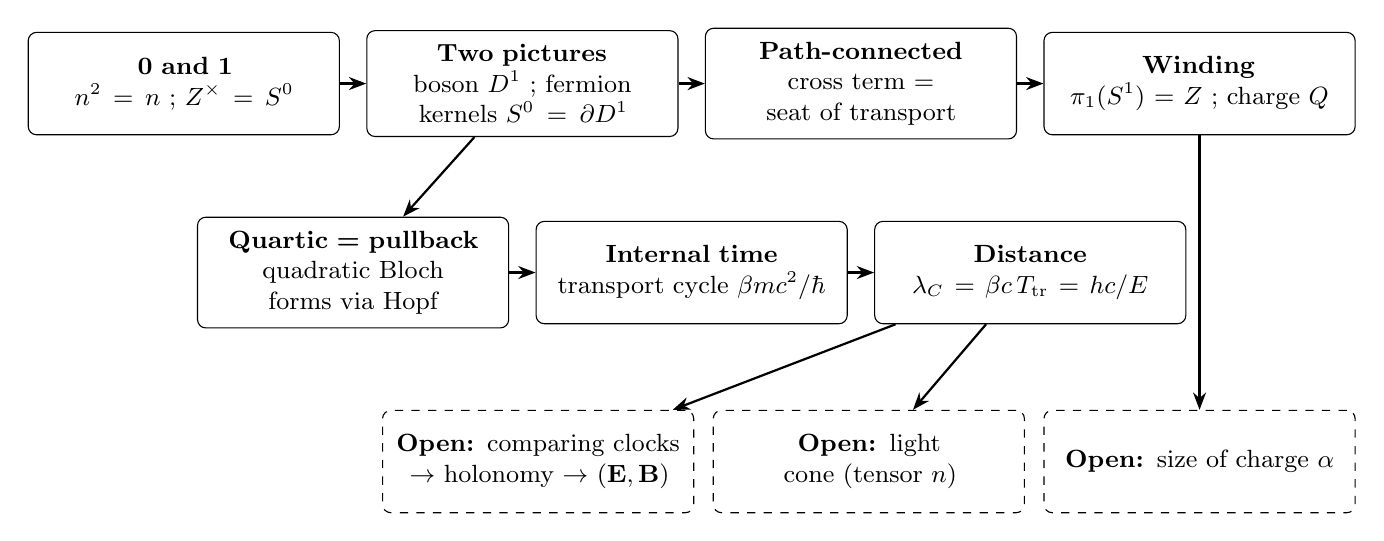
\begin{tikzpicture}[
  box/.style={draw, rounded corners=3pt, align=center, font=\small, inner sep=5pt, text width=3.6cm, minimum height=1.3cm},
  open/.style={box, dashed},
  arr/.style={-{Stealth[length=2.2mm]}, thick}]
\node[box] (a) at (0,0) {\textbf{0 and 1}\\ $n^2=n$ ; $\mathbb{Z}^{\times}=S^0$};
\node[box] (b) at (4.3,0) {\textbf{Two pictures}\\ boson $D^1$ ; fermion kernels $S^0=\partial D^1$};
\node[box] (c) at (8.6,0) {\textbf{Path-connected}\\ cross term = seat of transport};
\node[box] (d) at (12.9,0) {\textbf{Winding}\\ $\pi_1(S^1)=\mathbb{Z}$ ; charge $Q$};
\node[box] (e) at (2.15,-2.4) {\textbf{Quartic = pullback}\\ quadratic Bloch forms via Hopf};
\node[box] (f) at (6.45,-2.4) {\textbf{Internal time}\\ transport cycle $\beta mc^2/\hbar$};
\node[box] (g) at (10.75,-2.4) {\textbf{Distance}\\ $\lambda_C=\beta c\,T_{\mathrm{tr}}=hc/E$};
\node[open] (h) at (12.9,-4.8) {\textbf{Open:} size of charge $\alpha$};
\node[open] (i) at (4.5,-4.8) {\textbf{Open:} comparing clocks $\to$ holonomy $\to$ $(\mathbf{E},\mathbf{B})$};
\node[open] (j) at (8.7,-4.8) {\textbf{Open:} light cone (tensor $n$)};
\draw[arr] (a) -- (b); \draw[arr] (b) -- (c); \draw[arr] (c) -- (d);
\draw[arr] (b) -- (e); \draw[arr] (e) -- (f); \draw[arr] (f) -- (g);
\draw[arr] (d) -- (h); \draw[arr] (g) -- (i); \draw[arr] (g) -- (j);
\end{tikzpicture}
\caption{\textbf{The flow of the argument}}
\label{fig:flow}
\vspace{0.4em}
\begin{minipage}{0.95\textwidth}
\justifying\small
Top row: the integer thread, from the arithmetic of $0$ and $1$ (Sec.~\ref{sec:arith}) through the two solution sets (Sec.~\ref{sec:twopictures}) and path-connectedness (Sec.~\ref{sec:path}) to the winding number identified with charge (Sec.~\ref{sec:winding}). Middle row: the energy and time thread, from the quartic as a Hopf pullback (Sec.~\ref{sec:quartic}) to the internal time and to distance built from it (Sec.~\ref{sec:time}). Bottom row, dashed: what is not derived here; the size of the charge hangs below the winding thread, while clock comparison and the light cone hang below distance, where the metric enters (Sec.~\ref{sec:metric}).
\end{minipage}
\end{figure*}

% =====================================================================
\appendix

\section{Numerical Verification}
\label{app:numeric}

Every analytic claim was checked numerically. The script below reproduces the checks: (1) the solution sets of Proposition~\ref{prop:sets} and the roots of $\binom{p}{3}$; (2)--(3) the first-order equation, the equal-weight decomposition and $\langle H\rangle=0$; (4) the quadratic Bloch forms and Proposition~\ref{prop:quartic}; (5) the Wronskian charge $Q=\pm1$; (6) the closed form $W=\chi_4(q)$ for coprime odd pairs below $40$; (7) $\beta$ from $a_e$, the ratio $\beta$ between the two clocks, and $\lambda_C=\beta c\,T_{\mathrm{tr}}$.

\begin{lstlisting}[caption={Verification of Propositions~\ref{prop:sets} and~\ref{prop:quartic}, Theorem~\ref{thm:equiv}, Eq.~\eqref{eq:wronskian}, and Tables~\ref{tab:charge}--\ref{tab:clocks}.}]
import numpy as np, math
sx=np.array([[0,1],[1,0]]); sy=np.array([[0,-1j],[1j,0]]); sz=np.array([[1,0],[0,-1]])
w=1.0; E0=1.0
chi=lambda t: np.array([np.cos(w*t/2), np.sin(w*t/2)], dtype=complex)

# (1) kernel terms alone give 1 only at the ends of the segment
x=np.linspace(0,1,100001)
for p in [1.5,2,3]:
    f=x**p+(1-x)**p
    assert np.all(f[1:-1]<1) and f[0]==1 and f[-1]==1
assert sorted(np.round(np.roots([1,-3,2,0]).real,12))==[0,1,2]

# (2) first-order equation and eigenvalues of H
dt=1e-6
for t in np.linspace(0.1,5,7):
    d=(chi(t+dt)-chi(t-dt))/(2*dt)
    assert np.max(np.abs(1j*d-(w/2)*sy@chi(t)))<1e-6
assert np.allclose(np.linalg.eigvalsh((w/2)*sy),[-0.5,0.5])

# (3) equal-weight decomposition, <H>=0
vals,V=np.linalg.eigh((w/2)*sy)
for t in np.linspace(0,2*np.pi,9):
    c=V.conj().T@chi(t)
    assert np.allclose(np.abs(c)**2,[0.5,0.5])
    assert abs((chi(t).conj()@((w/2)*sy)@chi(t)).real)<1e-12

# (4) quadratic Bloch forms; quartic derived from three inputs
for t in np.linspace(0,2*np.pi,50):
    c=chi(t); Sx=(c.conj()@sx@c).real; Sz=(c.conj()@sz@c).real
    assert abs(E0*np.cos(w*t/2)**4-E0*((1+Sz)/2)**2)<1e-12
    assert abs(0.5*E0*np.sin(w*t)**2-0.5*E0*Sx**2)<1e-12
    KE=0.5*E0*Sx**2; s=E0-KE; d=-E0*Sz
    assert abs((s-d)/2-E0*np.cos(w*t/2)**4)<1e-12

# (5) Wronskian charge: +1 for the rotor, -1 reversed
t=np.linspace(0,10,1001); a=np.cos(w*t/2); b=np.sin(w*t/2)
ad=-(w/2)*np.sin(w*t/2); bd=(w/2)*np.cos(w*t/2)
assert np.allclose((2/w)*(a*bd-b*ad),1)
assert np.allclose((2/w)*(a*(-bd)-(-b)*ad),-1)

# (6) winding number W = chi_4(q) for coprime odd p:q
def chi4(n): return 0 if n%2==0 else (1 if n%4==1 else -1)
def W(p,q): return 0.5*sum((-1)**k*math.copysign(1,
    math.sin(math.pi*q*(2*k+1)/(2*p))) for k in range(2*p))
for p in range(1,40,2):
    for q in range(1,40,2):
        if math.gcd(p,q)==1: assert W(p,q)==chi4(q)

# (7) beta from a_e; two clocks differ by beta; distance = speed x tick
ae=0.00115965218059
beta=math.sqrt(1-1/(1+ae/math.sqrt(2))**2)
h=6.62607015e-34; c=299792458; me=9.1093837015e-31
lamC=h/(me*c); nu_branch=me*c**2/h; nu_tr=beta*c/lamC
assert abs(nu_tr/nu_branch-beta)<1e-15
assert abs(beta*c/nu_tr-lamC)<1e-25
print(f"beta={beta:.7f} nu_tr={nu_tr:.5e} Hz")
print("all checks passed")
\end{lstlisting}

\section{The Bloch Map and the Derivation of the Quartic}
\label{app:bloch}

\paragraph{Half-angle to full-angle.} For the rotor~\eqref{eq:rotor}, the occupations are $n_{A,B}=\tfrac12(1\pm\cos\omega t)$ by the half-angle formulas, so $s_z=n_A-n_B=\cos\omega t$ and, from $2\cos\phi\sin\phi=\sin2\phi$, $s_x=\sin\omega t$; $s_y=0$ because $\chi$ is real. The rotor advances by $\omega t/2$, the Bloch vector by $\omega t$: this is the two-to-one map.

\paragraph{Uniqueness.} The two equations of the proof of Proposition~\ref{prop:quartic}, the sum fixed by conservation and the oscillator energy and the difference fixed by the energy gradient, determine $T_A$ and $T_B$ separately. The coefficient structure $\tfrac14(1\pm s_z)^2$ shows that the fourth power in $\chi$ is the square of an occupation that is linear in $s_z$.

\paragraph{The boson in the same language.} Squaring the bosonic identity~\eqref{eq:boson} at the half angle reproduces the fermionic identity, with cross term $2\sin^2(\theta/2)\cos^2(\theta/2)=\tfrac12\sin^2\theta$. The fourth power and the transit seat are what the second squaring adds; the sign flip under $\theta\to\theta+2\pi$ is already present at the first.

\section{Words That Split in Two}
\label{app:words}

Several words borrowed from established fields carry two meanings in this paper. When a reader's objection seems to miss the point, the first thing to check is whether the same word is being read in the other sense.

\paragraph{Occupation number.} Here: the share $n_A=\cos^2(\theta/2)$ of the energy held by kernel $A$, a continuous quantity. In standard theory: the eigenvalue $0$ or $1$ of the fermion number operator. Both satisfy the idempotent equation~\eqref{eq:idem} at the ends, but they are different objects.

\paragraph{Proper time.} Here: the internal clock carried by the particle, the transport cycle. In general relativity: the length of a worldline given by the metric. Section~\ref{sec:time} argues that the first runs proportionally to the second, which is a claim, not a definition.

\paragraph{Radiation.} Here: the transfer of energy between the two kernels. In electromagnetism: emission of electromagnetic waves to infinity. ``Time stops when radiation stops'' refers to the first.

\paragraph{Double cover.} Here: the sign flip of the real amplitude after one turn. In standard theory also: the covering $SU(2)\to SO(3)$ of spatial rotations. Whether the two coincide is the open question of Sec.~\ref{sec:limits}.

\paragraph{Hidden variable.} Here: a degree of freedom absent from the standard formalism, carried by the particle, as density is carried by a particle in smoothed-particle hydrodynamics. In the Bell literature: a local variable meant to explain two-particle correlations. This paper uses only the first sense.

% =====================================================================
\begin{thebibliography}{99}

\bibitem{ref:p1}
S.~Hanamura,
\emph{A Model of an Electron Including Two Perfect Black Bodies},
Zenodo (2018), \href{https://doi.org/10.5281/zenodo.16759284}{10.5281/zenodo.16759284}.

\bibitem{ref:p7}
S.~Hanamura,
\emph{Coexistence of Positive- and Negative-Energy States in the Dirac Framework within the 0-Sphere Model},
Zenodo, \href{https://doi.org/10.5281/zenodo.17760132}{10.5281/zenodo.17760132}.

\bibitem{ref:p10}
S.~Hanamura,
\emph{Redefining Electron Spin and Anomalous Magnetic Moment Through Harmonic Oscillation and Lorentz Contraction},
Zenodo (2024), \href{https://doi.org/10.5281/zenodo.17764997}{10.5281/zenodo.17764997}.

\bibitem{ref:p20}
S.~Hanamura,
\emph{Emergent Conservation Laws from Internal Geometry: A Noetherian Reinterpretation in the 0-Sphere Model},
Zenodo (2025), \href{https://doi.org/10.5281/zenodo.17765244}{10.5281/zenodo.17765244}.

\bibitem{ref:p24}
S.~Hanamura,
\emph{Thermal Geodesics in the 0-Sphere Model: Extending General Relativity through Internal Thermodynamic Structure},
Zenodo (2025), \href{https://doi.org/10.5281/zenodo.17765349}{10.5281/zenodo.17765349}.

\bibitem{ref:p33}
S.~Hanamura,
\emph{Geometrical Confinement of Energy in the 0-Sphere Model: A Topological Mechanism Underlying Rest Mass and Zitterbewegung},
Zenodo (2026), \href{https://doi.org/10.5281/zenodo.18356895}{10.5281/zenodo.18356895}.

\bibitem{ref:p38}
S.~Hanamura,
\emph{Electron Interference from Internal Geometry: Two-Kernel SU(2) Structure, Quartic Energy Flow, and an Intrinsic Visibility Limit},
Zenodo (2026), \href{https://doi.org/10.5281/zenodo.18718174}{10.5281/zenodo.18718174}.

\bibitem{ref:p43}
S.~Hanamura,
\emph{On Observer-Dependent Torsion, Zitterbewegung, and Phase Accumulation in the 0-Sphere Model},
Zenodo, \href{https://doi.org/10.5281/zenodo.18896784}{10.5281/zenodo.18896784}.

\bibitem{ref:p46}
S.~Hanamura,
\emph{Geometric Origin of the One-Half Factor: Thermal Potential Energy Floor and Zero-Point Energy in the 0-Sphere Model},
Zenodo, \href{https://doi.org/10.5281/zenodo.19010945}{10.5281/zenodo.19010945}.

\bibitem{ref:p51}
S.~Hanamura,
\emph{Helical Trajectory, Fixed-Endpoint Line Integrals, and the Emergence of the Spacetime Metric in the 0-Sphere Model},
Zenodo (2026), \href{https://doi.org/10.5281/zenodo.20388056}{10.5281/zenodo.20388056}.

\bibitem{ref:p68}
S.~Hanamura,
\emph{The 0-Sphere Model: A Structural Overview},
Zenodo (2026), in preparation.

\bibitem{ref:hehl}
F.~W.~Hehl and Yu.~N.~Obukhov,
\emph{Foundations of Classical Electrodynamics: Charge, Flux, and Metric}
(Birkh\"auser, Boston, 2003).

\bibitem{ref:schrodinger}
E.~Schr\"odinger,
\emph{\"Uber die kr\"aftefreie Bewegung in der relativistischen Quantenmechanik},
Sitzungsber.~Preuss.~Akad.~Wiss.~Phys.-Math.~Kl.\ \textbf{24}, 418 (1930).

\bibitem{ref:fw}
L.~L.~Foldy and S.~A.~Wouthuysen,
\emph{On the Dirac Theory of Spin 1/2 Particles and Its Non-Relativistic Limit},
Phys.~Rev.\ \textbf{78}, 29 (1950).

\bibitem{ref:thaller}
B.~Thaller,
\emph{The Dirac Equation}
(Springer, Berlin, 1992).

\end{thebibliography}

\end{document}
